\documentclass[a4paper,11pt]{report}
\usepackage[utf8]{inputenc}
\usepackage[T1]{fontenc}
\usepackage{lmodern}
\usepackage[ngerman]{babel}
\usepackage[margin=20mm, left=20mm, right=10mm, headheight=15pt, includeheadfoot]{geometry}
\usepackage{fancyhdr}
\usepackage{opensans}
\usepackage{titlesec}
\usepackage{tocloft}
\usepackage{titling}
\usepackage{hyperref}
\usepackage{graphicx}
\usepackage{enumerate}
\usepackage{float}
\usepackage{caption}
\usepackage{listings}
\usepackage{minted}
\usepackage{subcaption}
\usepackage{enumitem}
\usemintedstyle{vs}

% Author and subject
\author{Felix Hillebrand}
\newcommand{\subject}{SSD4UE}

\graphicspath{ {./images/} {./notebooks/assets/aufgabe_01 } {./notebooks/assets/aufgabe_02 } {./notebooks/assets/aufgabe_03 } {./notebooks/assets/aufgabe_04 } {./notebooks/assets/aufgabe_05 } {./notebooks/assets/aufgabe_06 }}

% Set default font to OpenSans
\renewcommand*\familydefault{\sfdefault}

% Page style for cover page
\fancypagestyle{cover}{
    \fancyhf{}
    \renewcommand{\headrulewidth}{0pt}
    \renewcommand{\footrulewidth}{0pt}
}

% Page style for main content
\fancypagestyle{main}{
    \fancyhf{}
    \fancyhead[L]{\theauthor}
    \fancyhead[R]{\subject}
    \fancyfoot[C]{\thepage}
    \renewcommand{\headrulewidth}{0.4pt}
    \renewcommand{\footrulewidth}{0pt}
}

\titleformat{\chapter}[block]
  {\normalfont\Large\bfseries} % change \Large to \large or any other size that fits
  {\thechapter}
  {1em}
  {}

  \titlespacing*{\chapter}{0pt}{*4}{*2.5}

% Cover page
\newcommand{\coverpage}{
    \thispagestyle{cover}
    \begin{center}
        % {
\includegraphics[height=3cm]{fh-logo.png}}\\[1cm]
        {\LARGE \thetitle}\\[0.5cm]
        {\large \theauthor}\\
        \href{mailto:97hilfel@gmail.com}{97hilfel@gmail.com}\\
    \end{center}
    \tableofcontents
    \clearpage
}

\newcommand{\screenshot}[1]{
    \begin{figure}[H]
        \centering
        \includegraphics[scale=0.375]{#1}
    \end{figure}
}

% Main document
\begin{document}

% Color definitions
\definecolor{LightGray}{gray}{0.9}
\definecolor{DarkGray}{gray}{0.3}

\title{AMS4~-~U02}
\coverpage

\pagenumbering{roman}
\clearpage
\pagenumbering{arabic}
\pagestyle{main}

\chapter{Bipartite Graphen}
    \begin{description}
        \item[Aufgabe:] Bestimmen Sie für die Graphen A, B und C ob es sich um bipartite Graphen handelt, und geben sie falls möglich zei Knotenmegen an. \hfill
        \begin{figure}[htbp]
            \centering
            \begin{subfigure}[b]{0.3\textwidth}
                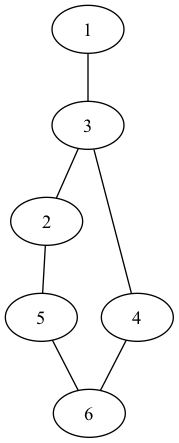
\includegraphics[height=0.2\textheight]{images/A}
                \caption{A}
                \label{fig:a01_a}
            \end{subfigure}
            \hfill
            \begin{subfigure}[b]{0.3\textwidth}
                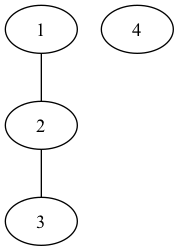
\includegraphics[height=0.2\textheight]{images/B}
                \caption{B}
                \label{fig:a01_b}
            \end{subfigure}
            \hfill
            \begin{subfigure}[b]{0.3\textwidth}
                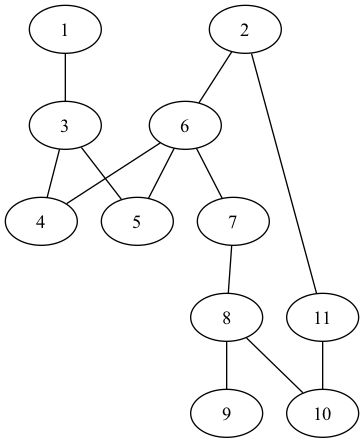
\includegraphics[height=0.2\textheight]{images/C}
                \caption{C}
                \label{fig:a01_c}
            \end{subfigure}
            \hfill
        \end{figure}
        \item[Lösung:] \hfill \newline % Use hfill to move the figure to the next line
        \begin{figure}[htbp]
            \centering
            \begin{subfigure}[b]{0.3\textwidth}
                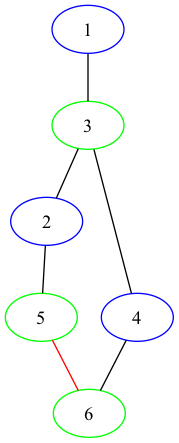
\includegraphics[height=0.2\textheight]{images/A_colored}
                \caption{A - nicht Bipartit - Kante $\{5, 6\}$}
                \label{fig:a01_a_colored}
            \end{subfigure}
            \hfill
            \begin{subfigure}[b]{0.3\textwidth}
                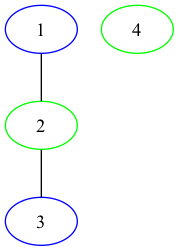
\includegraphics[height=0.2\textheight]{images/B_colored}
                \caption{B - Bipartit}
                \label{fig:a01_b_colored}
            \end{subfigure}
            \hfill
            \begin{subfigure}[b]{0.3\textwidth}
                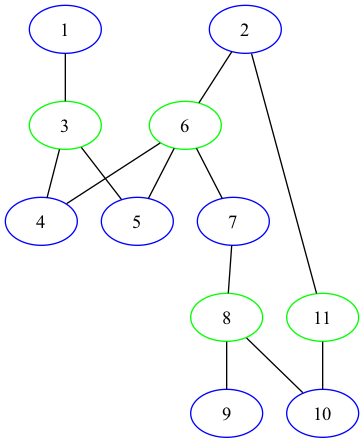
\includegraphics[height=0.2\textheight]{images/C_colored}
                \caption{C - Bipartit}
                \label{fig:a01_c_colored}
            \end{subfigure}
            \hfill
        \end{figure}

    \end{description}
\newpage

\chapter{Topologisches Sortieren}
Ein prominentes Beispiel für das Erkennen von Zyklen ist das Serialisieren von Transaktionen in Datenbanksystemen.
In der untenstehenden Tabelle ist der vom DBMS registrierte Ablaufplan angegeben.
Transformieren Sie den Plan in einen gerichteten Graphen, der die Abhängigkeiten zwischen den Transaktionen abbildet und ermitteln Sie ob ein äquivalenter serieller Ablaufplan
(Serie von Transaktionen ohne Verzahnung)
existiert und geben Sie gegeben falls einen möglichen an.

\textbf{Hinweis}: Gegeben 2 Transaktionen \texttt{a} und \texttt{b} $a != b$ und eine Tabelle X so gilt:

\begin{itemize}
    \item wenn \texttt{(R, a, X)} vor \texttt{(W, b, X)} dann \texttt{a} vor \texttt{b} im seriellen Plan)
    \item wenn \texttt{(W, a, X)} vor \texttt{(R, b, X)} dann \texttt{a} vor \texttt{b} im seriellen Plan)
    \item wenn \texttt{(W, a, X)} vor \texttt{(W, b, X)} dann \texttt{a} vor \texttt{b} im seriellen Plan)
\end{itemize}

\begin{table}[htbp]
    \begin{tabular}{|l|l|l|l|}
        \hline
        Id & AT & Tx & Table \\ \hline
        1  & R  & 1  & A     \\ \hline
        2  & W  & 1  & A     \\ \hline
        3  & R  & 7  & B     \\ \hline
        4  & R  & 2  & A     \\ \hline
        5  & W  & 2  & A     \\ \hline
        6  & R  & 1  & B     \\ \hline
        7  & W  & 1  & B     \\ \hline
        8  & R  & 2  & B     \\ \hline
        9  & W  & 2  & B     \\ \hline
        10 & R  & 3  & A     \\ \hline
        11 & W  & 4  & A     \\ \hline
        12 & R  & 5  & B     \\ \hline
        13 & R  & 1  & C     \\ \hline
        14 & R  & 6  & C     \\ \hline
        15 & W  & 8  & A     \\ \hline
        16 & W  & 8  & B     \\ \hline
    \end{tabular}
\end{table}

Abhängigkeiten für Tabelle \texttt{A}:

\begin{itemize}
    \item \texttt{(R, 1, A)} vor \texttt{(W, 2, A)}: Tx \texttt{1} $\rightarrow$ Tx \texttt{2}
    \item \texttt{(W, 1, A)} vor \texttt{(R, 2, A)}: Tx \texttt{1} $\rightarrow$ Tx \texttt{2}
    \item \texttt{(W, 1, A)} vor \texttt{(R, 3, A)}: Tx \texttt{1} $\rightarrow$ Tx \texttt{3}
    \item \texttt{(W, 1, A)} vor \texttt{(W, 4, A)}: Tx \texttt{1} $\rightarrow$ Tx \texttt{4}
    \item \texttt{(W, 1, A)} vor \texttt{(W, 8, A)}: Tx \texttt{1} $\rightarrow$ Tx \texttt{8}
    \item \texttt{(W, 2, A)} vor \texttt{(R, 3, A)}: Tx \texttt{2} $\rightarrow$ Tx \texttt{3}
    \item \texttt{(W, 2, A)} vor \texttt{(W, 4, A)}: Tx \texttt{2} $\rightarrow$ Tx \texttt{4}
    \item \texttt{(W, 2, A)} vor \texttt{(W, 8, A)}: Tx \texttt{2} $\rightarrow$ Tx \texttt{8}
\end{itemize}

Abhängigkeiten für Tabelle \texttt{B}:

\begin{itemize}
    \item \texttt{(R, 7, B)} vor \texttt{(W, 1, B)}: Tx \texttt{7} $\rightarrow$ Tx \texttt{1}
    \item \texttt{(R, 1, B)} vor \texttt{(W, 2, B)}: Tx \texttt{1} $\rightarrow$ Tx \texttt{2}
    \item \texttt{(W, 1, B)} vor \texttt{(R, 2, B)}: Tx \texttt{1} $\rightarrow$ Tx \texttt{2}
    \item \texttt{(W, 1, B)} vor \texttt{(R, 5, B)}: Tx \texttt{1} $\rightarrow$ Tx \texttt{5}
    \item \texttt{(W, 1, B)} vor \texttt{(W, 8, B)}: Tx \texttt{1} $\rightarrow$ Tx \texttt{8}
    \item \texttt{(W, 2, B)} vor \texttt{(R, 5, B)}: Tx \texttt{2} $\rightarrow$ Tx \texttt{5}
    \item \texttt{(W, 2, B)} vor \texttt{(W, 8, B)}: Tx \texttt{2} $\rightarrow$ Tx \texttt{8}
    \item \texttt{(R, 5, B)} vor \texttt{(W, 8, B)}: Tx \texttt{5} $\rightarrow$ Tx \texttt{8}
\end{itemize}

Abhängigkeiten für Tabelle \texttt{C}:

Es gibt keine schreioperationen für Tabelle \texttt{C}

\begin{figure}[htbp]
    \centering
    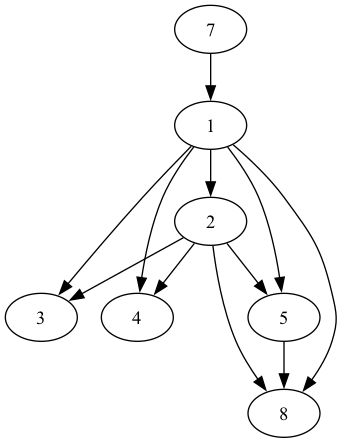
\includegraphics[height=0.2\textheight]{images/dependency_graph}
    \caption{Dependency Graph}
    \label{fig:a02_dependency_graph}
\end{figure}

\newpage

\chapter{Scheduling (Partnerarbeit)}

Aurora hat ein Problem: Sie hat heute einige Aufgabe zu erledigen, aber keine echte Lust dazu.

In \texttt{Precedences.dot} finden Sie einen Graphen, der die Reihenfolgenbedingung der heutigen Tätigkeiten beinhaltet.
Zusätzlich benötigen Aufgaben, wenn sie an anderen Orten in der Wohnung erledigt, werden unterschiedlich viel Zeit.
Diese Informaionen entnehmen Sie \texttt{Costs.dot}.
Die Kosten die Aurora aufwenden muss, um von einem ort zum anderen zu kommen finden Sie in \texttt{Places.dot}.

(Achten Sie beim Enlesen auf das Encoding/Umlaute und ob die Gewichte auch wirklich als Zahlen interpretiert werden)

Nutzen Sie einen geeigneten Algorithmus (tiefensuche, Breitensuche, Branch-Bound, etc.) um die günstigste Lösung für Auroras Problem zu finden.

\chapter{Snake}

Ein Optimaler Snake-Spieler, der Garantiert die maximale Punkte Anuzahl erreichen möchte, wählt einen Hamilton Zyklus auf dem Spielfeld und folgt diesem stur, bis die Schlange die maximale Länge erreicht hat, ohne sich von Futterknoten (schwarz) ablenken zu lassen (da er/sie sie sicher reichen wird).
Finen Sie wenn möglich für beide Spielfelder einen Solchen Zyklus (beginnend in der linken operen Ecke) oder begründen Sie, warum dieser nicht existiert.

\newpage

\chapter{Kürzeste Wege Djikstra vs A*}

Finden Sie den kürzesten Weg von Kloten \texttt{s} zu Knoten \texttt{z} mit Hilfe des Djikstra und A* Algorithmus.
Geben Sie das Ergebnis (Länge und kürzester Weg) sowie die Zustände der Variablen F, dist, und W am beginn jeder Schleife und am Ende des Algorithmus aus.
Die roten werte bei den Knoten entsprechen jener der Heursistik für diesen Knoten.

Wie viele Knoten expandiert (d.h. hinzufügen in F) der Algorithmus von Djikstra und wie viele der A*?

\section{Djikstra}\label{sec:djikstra}

\begin{minted}[
    frame=lines,
    framesep=2mm,
    baselinestretch=1.2,
    bgcolor=LightGray,
    linenos,
    breaklines
]{text}
F: {'s'} - dist: {'s': 0, 'a': inf, 'b': inf, 'c': inf, 'd': inf, 'e': inf, 'f': inf, 'g': inf, 'h': inf, 'i': inf, 'z': inf} - W: {'s': ['s'], 'a': [], 'b': [], 'c': [], 'd': [], 'e': [], 'f': [], 'g': [], 'h': [], 'i': [], 'z': []}
F: {'c', 's'} - dist: {'s': 0, 'a': 11, 'b': 10, 'c': 7, 'd': 7, 'e': 10, 'f': 8, 'g': inf, 'h': inf, 'i': inf, 'z': inf} - W: {'s': ['s'], 'a': ['s', 'a'], 'b': ['s', 'b'], 'c': ['s', 'c'], 'd': ['s', 'd'], 'e': ['s', 'e'], 'f': ['s', 'f'], 'g': [], 'h': [], 'i': [], 'z': []}
F: {'c', 'd', 's'} - dist: {'s': 0, 'a': 11, 'b': 10, 'c': 7, 'd': 7, 'e': 10, 'f': 8, 'g': inf, 'h': inf, 'i': 19, 'z': inf} - W: {'s': ['s'], 'a': ['s', 'a'], 'b': ['s', 'b'], 'c': ['s', 'c'], 'd': ['s', 'd'], 'e': ['s', 'e'], 'f': ['s', 'f'], 'g': [], 'h': [], 'i': ['s', 'c', 'i'], 'z': []}
F: {'c', 'd', 's', 'f'} - dist: {'s': 0, 'a': 11, 'b': 10, 'c': 7, 'd': 7, 'e': 10, 'f': 8, 'g': inf, 'h': inf, 'i': 19, 'z': inf} - W: {'s': ['s'], 'a': ['s', 'a'], 'b': ['s', 'b'], 'c': ['s', 'c'], 'd': ['s', 'd'], 'e': ['s', 'e'], 'f': ['s', 'f'], 'g': [], 'h': [], 'i': ['s', 'c', 'i'], 'z': []}
F: {'s', 'f', 'c', 'd', 'b'} - dist: {'s': 0, 'a': 11, 'b': 10, 'c': 7, 'd': 7, 'e': 10, 'f': 8, 'g': inf, 'h': inf, 'i': 19, 'z': inf} - W: {'s': ['s'], 'a': ['s', 'a'], 'b': ['s', 'b'], 'c': ['s', 'c'], 'd': ['s', 'd'], 'e': ['s', 'e'], 'f': ['s', 'f'], 'g': [], 'h': [], 'i': ['s', 'c', 'i'], 'z': []}
F: {'s', 'e', 'f', 'c', 'd', 'b'} - dist: {'s': 0, 'a': 11, 'b': 10, 'c': 7, 'd': 7, 'e': 10, 'f': 8, 'g': 29, 'h': inf, 'i': 19, 'z': inf} - W: {'s': ['s'], 'a': ['s', 'a'], 'b': ['s', 'b'], 'c': ['s', 'c'], 'd': ['s', 'd'], 'e': ['s', 'e'], 'f': ['s', 'f'], 'g': ['s', 'b', 'g'], 'h': [], 'i': ['s', 'c', 'i'], 'z': []}
F: {'a', 's', 'e', 'f', 'c', 'd', 'b'} - dist: {'s': 0, 'a': 11, 'b': 10, 'c': 7, 'd': 7, 'e': 10, 'f': 8, 'g': 29, 'h': inf, 'i': 19, 'z': inf} - W: {'s': ['s'], 'a': ['s', 'a'], 'b': ['s', 'b'], 'c': ['s', 'c'], 'd': ['s', 'd'], 'e': ['s', 'e'], 'f': ['s', 'f'], 'g': ['s', 'b', 'g'], 'h': [], 'i': ['s', 'c', 'i'], 'z': []}
F: {'a', 's', 'e', 'f', 'i', 'c', 'd', 'b'} - dist: {'s': 0, 'a': 11, 'b': 10, 'c': 7, 'd': 7, 'e': 10, 'f': 8, 'g': 29, 'h': inf, 'i': 19, 'z': inf} - W: {'s': ['s'], 'a': ['s', 'a'], 'b': ['s', 'b'], 'c': ['s', 'c'], 'd': ['s', 'd'], 'e': ['s', 'e'], 'f': ['s', 'f'], 'g': ['s', 'b', 'g'], 'h': [], 'i': ['s', 'c', 'i'], 'z': []}
F: {'a', 's', 'e', 'h', 'f', 'i', 'c', 'd', 'b'} - dist: {'s': 0, 'a': 11, 'b': 10, 'c': 7, 'd': 7, 'e': 10, 'f': 8, 'g': 29, 'h': 28, 'i': 19, 'z': 51} - W: {'s': ['s'], 'a': ['s', 'a'], 'b': ['s', 'b'], 'c': ['s', 'c'], 'd': ['s', 'd'], 'e': ['s', 'e'], 'f': ['s', 'f'], 'g': ['s', 'b', 'g'], 'h': ['s', 'c', 'i', 'h'], 'i': ['s', 'c', 'i'], 'z': ['s', 'c', 'i', 'z']}
F: {'a', 's', 'g', 'e', 'h', 'f', 'i', 'c', 'd', 'b'} - dist: {'s': 0, 'a': 11, 'b': 10, 'c': 7, 'd': 7, 'e': 10, 'f': 8, 'g': 29, 'h': 28, 'i': 19, 'z': 50} - W: {'s': ['s'], 'a': ['s', 'a'], 'b': ['s', 'b'], 'c': ['s', 'c'], 'd': ['s', 'd'], 'e': ['s', 'e'], 'f': ['s', 'f'], 'g': ['s', 'b', 'g'], 'h': ['s', 'c', 'i', 'h'], 'i': ['s', 'c', 'i'], 'z': ['s', 'c', 'i', 'h', 'z']}
F: {'a', 's', 'g', 'e', 'z', 'h', 'f', 'i', 'c', 'd', 'b'} - dist: {'s': 0, 'a': 11, 'b': 10, 'c': 7, 'd': 7, 'e': 10, 'f': 8, 'g': 29, 'h': 28, 'i': 19, 'z': 50} - W: {'s': ['s'], 'a': ['s', 'a'], 'b': ['s', 'b'], 'c': ['s', 'c'], 'd': ['s', 'd'], 'e': ['s', 'e'], 'f': ['s', 'f'], 'g': ['s', 'b', 'g'], 'h': ['s', 'c', 'i', 'h'], 'i': ['s', 'c', 'i'], 'z': ['s', 'c', 'i', 'h', 'z']}
\end{minted}

\texttt{F} wird um \textbf{10} Knoten expandiert.

\begin{figure}[htbp]
    \centering
    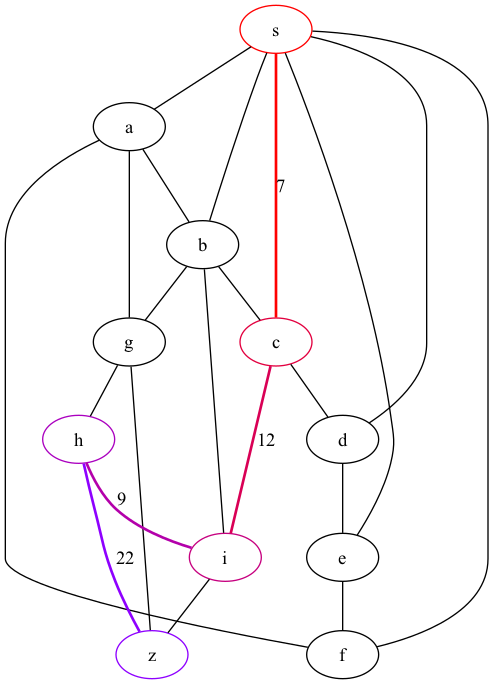
\includegraphics[height=0.2\textheight]{notebooks/assets/aufgabe_05/djikstra.png}
    \caption{Djkikstra}
    \label{fig:djkistra_graph}
\end{figure}

\section{A*}\label{sec:astar}

\begin{minted}[
    frame=lines,
    framesep=2mm,
    baselinestretch=1.2,
    bgcolor=LightGray,
    linenos,
    breaklines
]{text}
F: {'s'} - dist: {'s': 0, 'a': inf, 'b': inf, 'c': inf, 'd': inf, 'e': inf, 'f': inf, 'g': inf, 'h': inf, 'i': inf, 'z': inf} - W: {'s': ['s'], 'a': [], 'b': [], 'c': [], 'd': [], 'e': [], 'f': [], 'g': [], 'h': [], 'i': [], 'z': []}
F: {'b', 's'} - dist: {'s': 0, 'a': 11, 'b': 10, 'c': 7, 'd': 7, 'e': 10, 'f': 8, 'g': inf, 'h': inf, 'i': inf, 'z': inf} - W: {'s': ['s'], 'a': ['s', 'a'], 'b': ['s', 'b'], 'c': ['s', 'c'], 'd': ['s', 'd'], 'e': ['s', 'e'], 'f': ['s', 'f'], 'g': [], 'h': [], 'i': [], 'z': []}
F: {'c', 'b', 's'} - dist: {'s': 0, 'a': 11, 'b': 10, 'c': 7, 'd': 7, 'e': 10, 'f': 8, 'g': 29, 'h': inf, 'i': 22, 'z': inf} - W: {'s': ['s'], 'a': ['s', 'a'], 'b': ['s', 'b'], 'c': ['s', 'c'], 'd': ['s', 'd'], 'e': ['s', 'e'], 'f': ['s', 'f'], 'g': ['s', 'b', 'g'], 'h': [], 'i': ['s', 'b', 'i'], 'z': []}
F: {'c', 'b', 's', 'i'} - dist: {'s': 0, 'a': 11, 'b': 10, 'c': 7, 'd': 7, 'e': 10, 'f': 8, 'g': 29, 'h': inf, 'i': 19, 'z': inf} - W: {'s': ['s'], 'a': ['s', 'a'], 'b': ['s', 'b'], 'c': ['s', 'c'], 'd': ['s', 'd'], 'e': ['s', 'e'], 'f': ['s', 'f'], 'g': ['s', 'b', 'g'], 'h': [], 'i': ['s', 'c', 'i'], 'z': []}
F: {'s', 'h', 'i', 'c', 'b'} - dist: {'s': 0, 'a': 11, 'b': 10, 'c': 7, 'd': 7, 'e': 10, 'f': 8, 'g': 29, 'h': 28, 'i': 19, 'z': 51} - W: {'s': ['s'], 'a': ['s', 'a'], 'b': ['s', 'b'], 'c': ['s', 'c'], 'd': ['s', 'd'], 'e': ['s', 'e'], 'f': ['s', 'f'], 'g': ['s', 'b', 'g'], 'h': ['s', 'c', 'i', 'h'], 'i': ['s', 'c', 'i'], 'z': ['s', 'c', 'i', 'z']}
F: {'s', 'g', 'h', 'i', 'c', 'b'} - dist: {'s': 0, 'a': 11, 'b': 10, 'c': 7, 'd': 7, 'e': 10, 'f': 8, 'g': 29, 'h': 28, 'i': 19, 'z': 50} - W: {'s': ['s'], 'a': ['s', 'a'], 'b': ['s', 'b'], 'c': ['s', 'c'], 'd': ['s', 'd'], 'e': ['s', 'e'], 'f': ['s', 'f'], 'g': ['s', 'b', 'g'], 'h': ['s', 'c', 'i', 'h'], 'i': ['s', 'c', 'i'], 'z': ['s', 'c', 'i', 'h', 'z']}
F: {'s', 'g', 'z', 'h', 'i', 'c', 'b'} - dist: {'s': 0, 'a': 11, 'b': 10, 'c': 7, 'd': 7, 'e': 10, 'f': 8, 'g': 29, 'h': 28, 'i': 19, 'z': 50} - W: {'s': ['s'], 'a': ['s', 'a'], 'b': ['s', 'b'], 'c': ['s', 'c'], 'd': ['s', 'd'], 'e': ['s', 'e'], 'f': ['s', 'f'], 'g': ['s', 'b', 'g'], 'h': ['s', 'c', 'i', 'h'], 'i': ['s', 'c', 'i'], 'z': ['s', 'c', 'i', 'h', 'z']}
\end{minted}

\texttt{F} wird um \textbf{6} Knoten expandiert.

\begin{figure}[htbp]
    \centering
    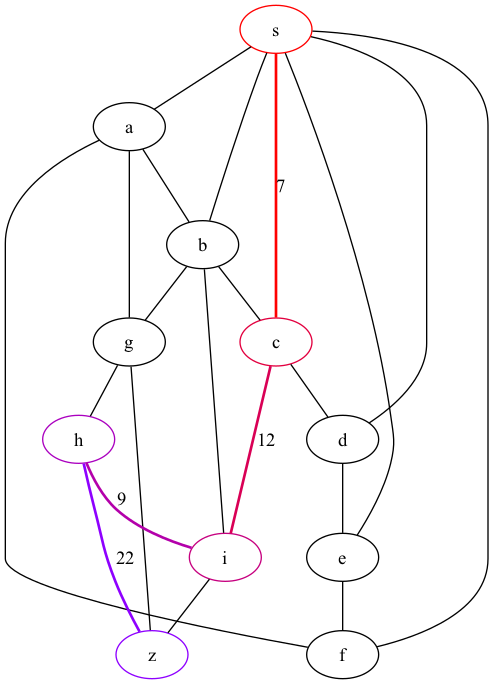
\includegraphics[height=0.2\textheight]{astar}
    \caption{A*}
    \label{fig:astar_graph}
\end{figure}

\newpage

\chapter{Ausflugsplanung (Partnerarbeit)}

Aurora und Aurelia planen ein kurzen Amerika Trip:
Sie müssen die Flughäfen Newark (\texttt{49611}), JFK (\texttt{212410}) und LaGuardia (\texttt{198373}) besuchen, um dort die Flughafensicherheit sowie die Mäusepopulation zu kontrollieren.
Da derzeit leider nur JFK mit Heißluftballon angeflogen werden kann, müssen Newark und LaGuardia zu Fuß erreicht werden.
Unterstützen Sie die beiden, indem Sie die kürzesten Wegen zwischen den Flughäfen mittels Djikstra Algorithmus ermitteln.
Sie finden ein Routingnetz in den Dateiimportfunktionen im \texttt{ipynb}.

Ermitteln Sie die paarweise kürzesten Wege und zeichnen Sie die kürzeste Rundreise.

\begin{figure}[htbp]
    \centering
    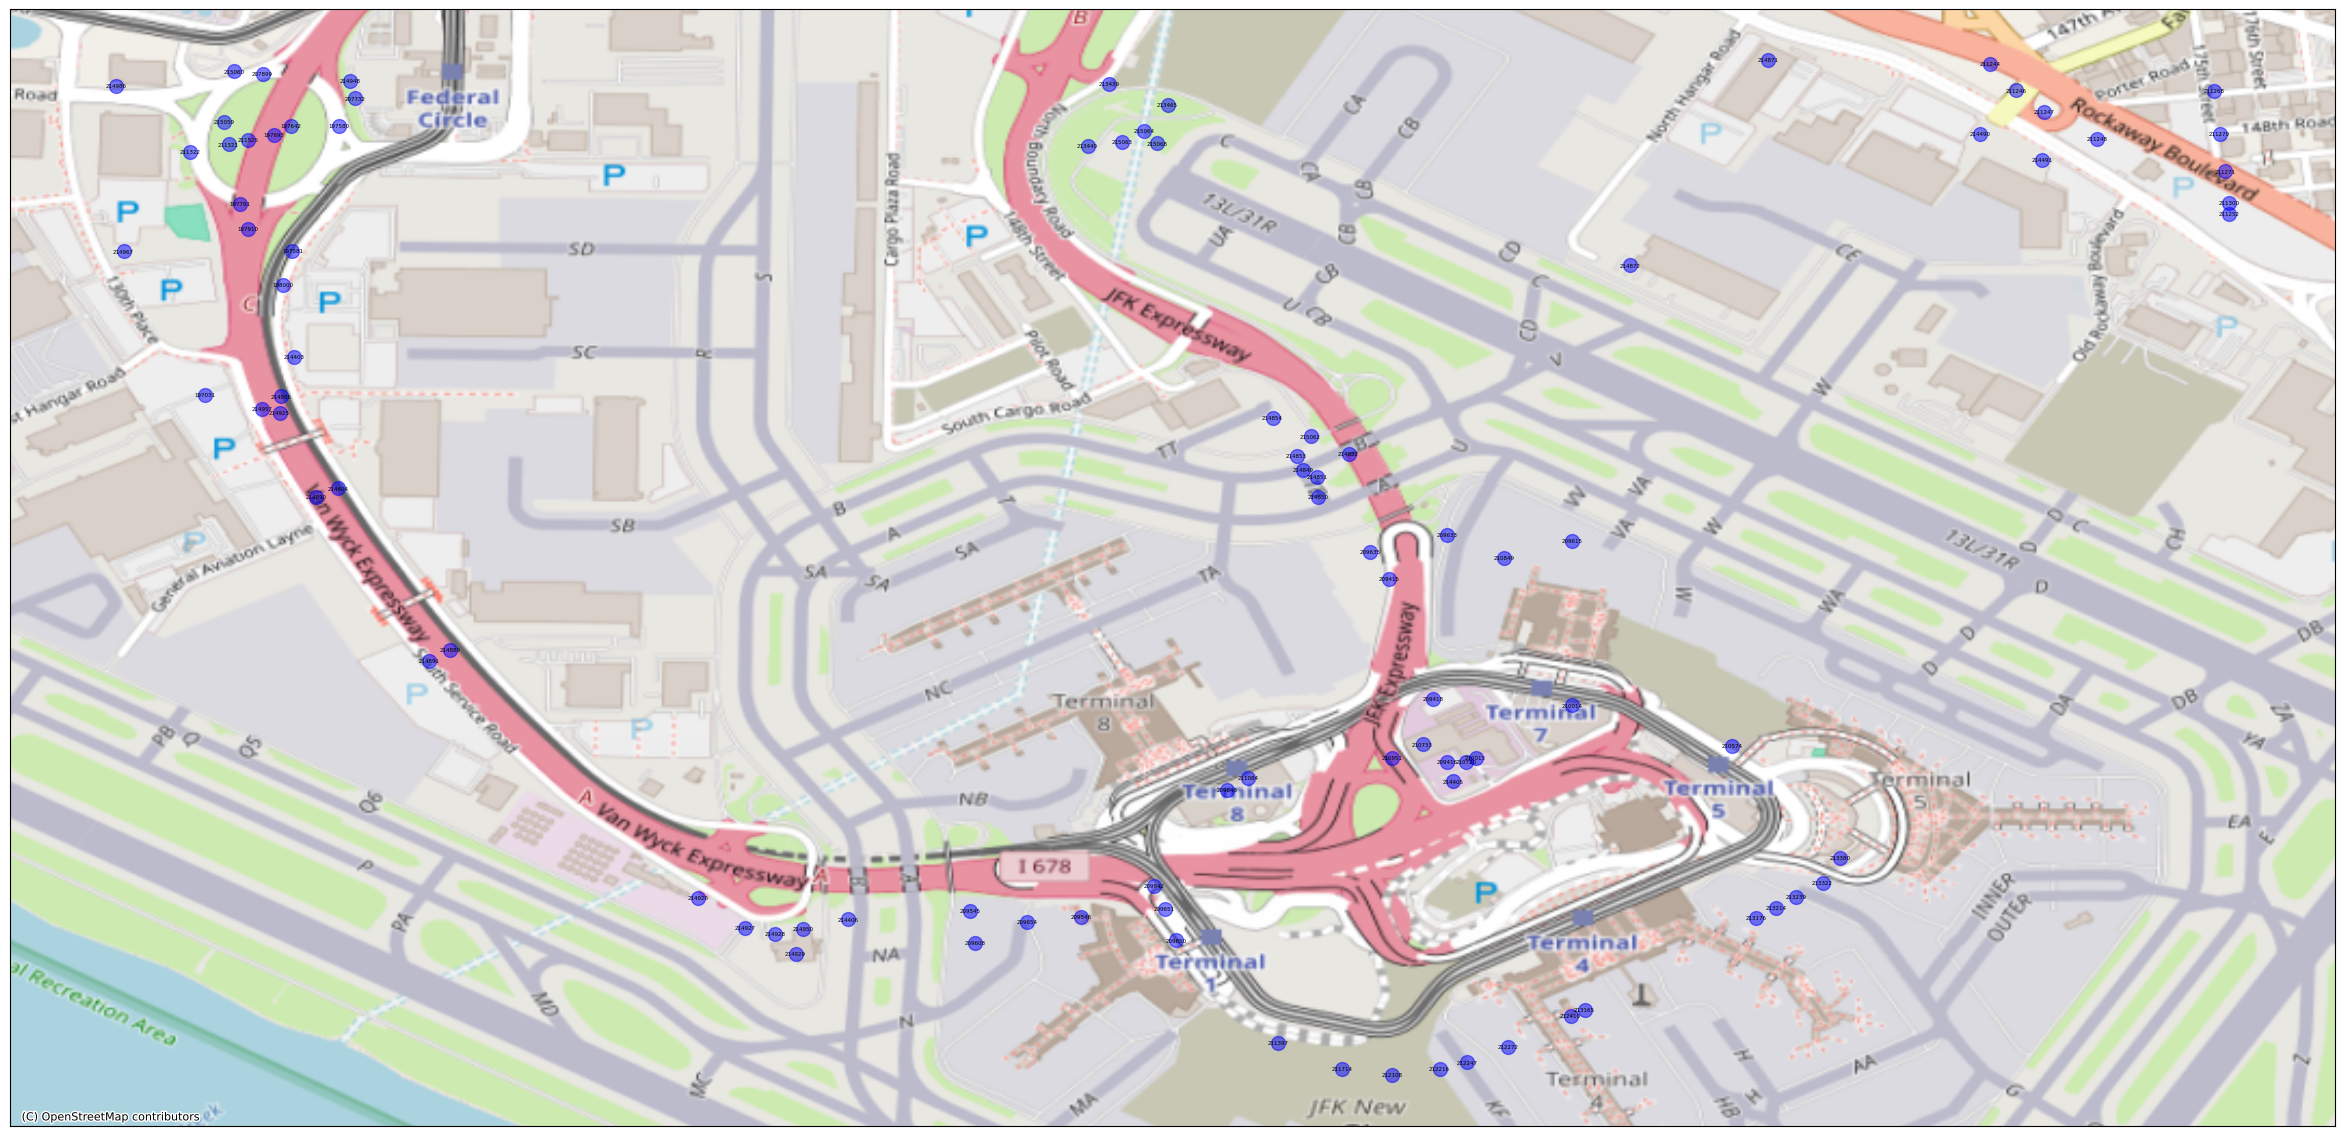
\includegraphics[width=3cm]{jfk}
    \caption{JFK}
    \label{fig:jfk}
\end{figure}

\begin{figure}[htbp]
    \centering
    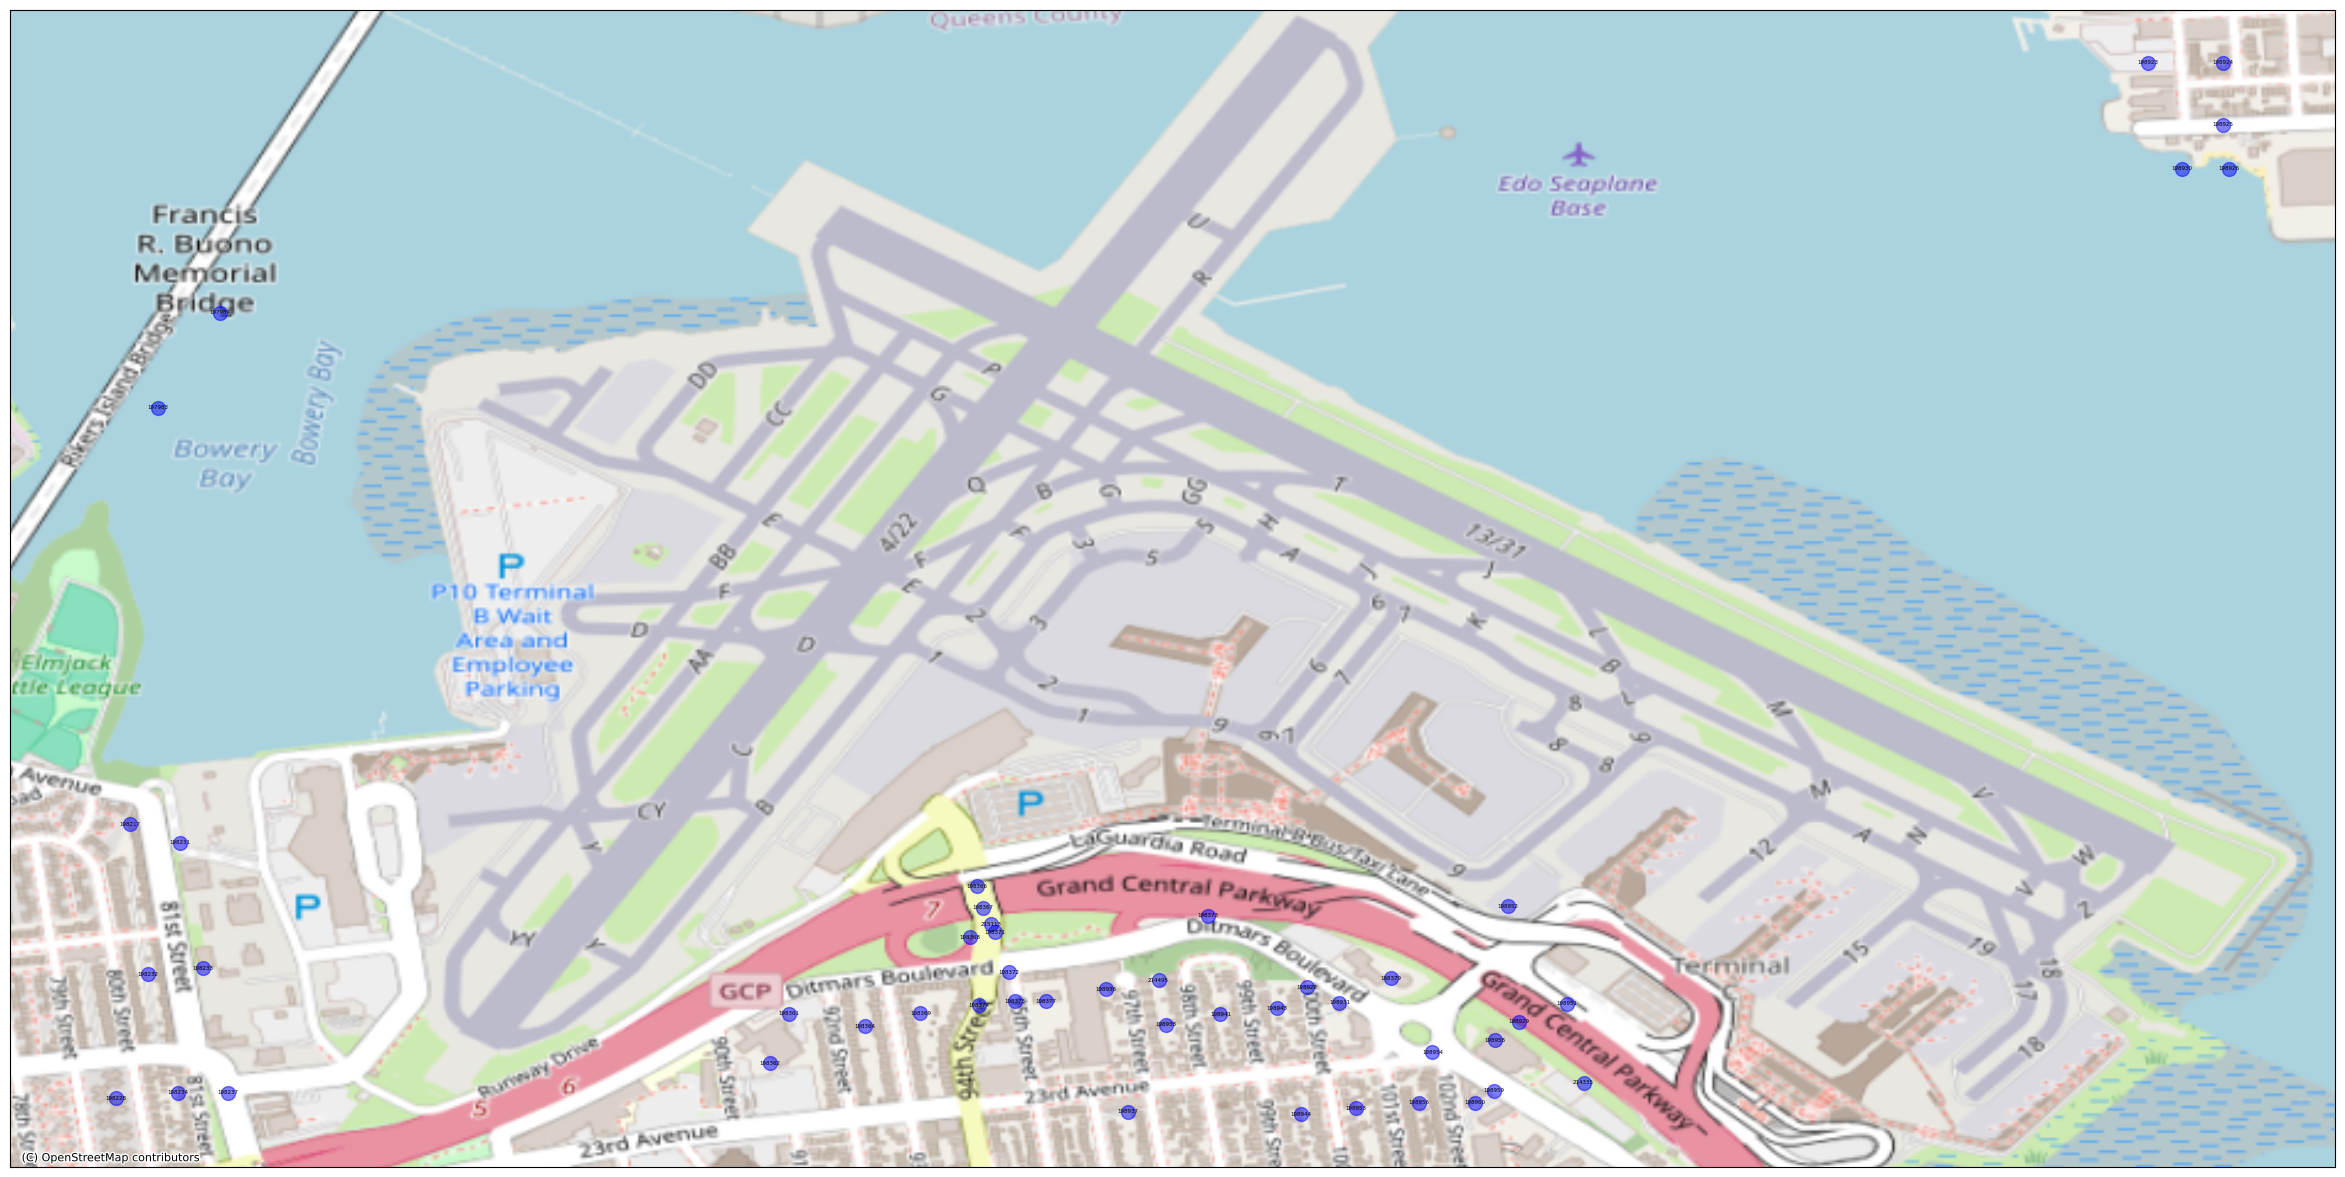
\includegraphics[width=3cm]{laguardia}
    \caption{LaGuardia}
    \label{fig:laguardia}
\end{figure}

\begin{figure}[htbp]
    \centering
    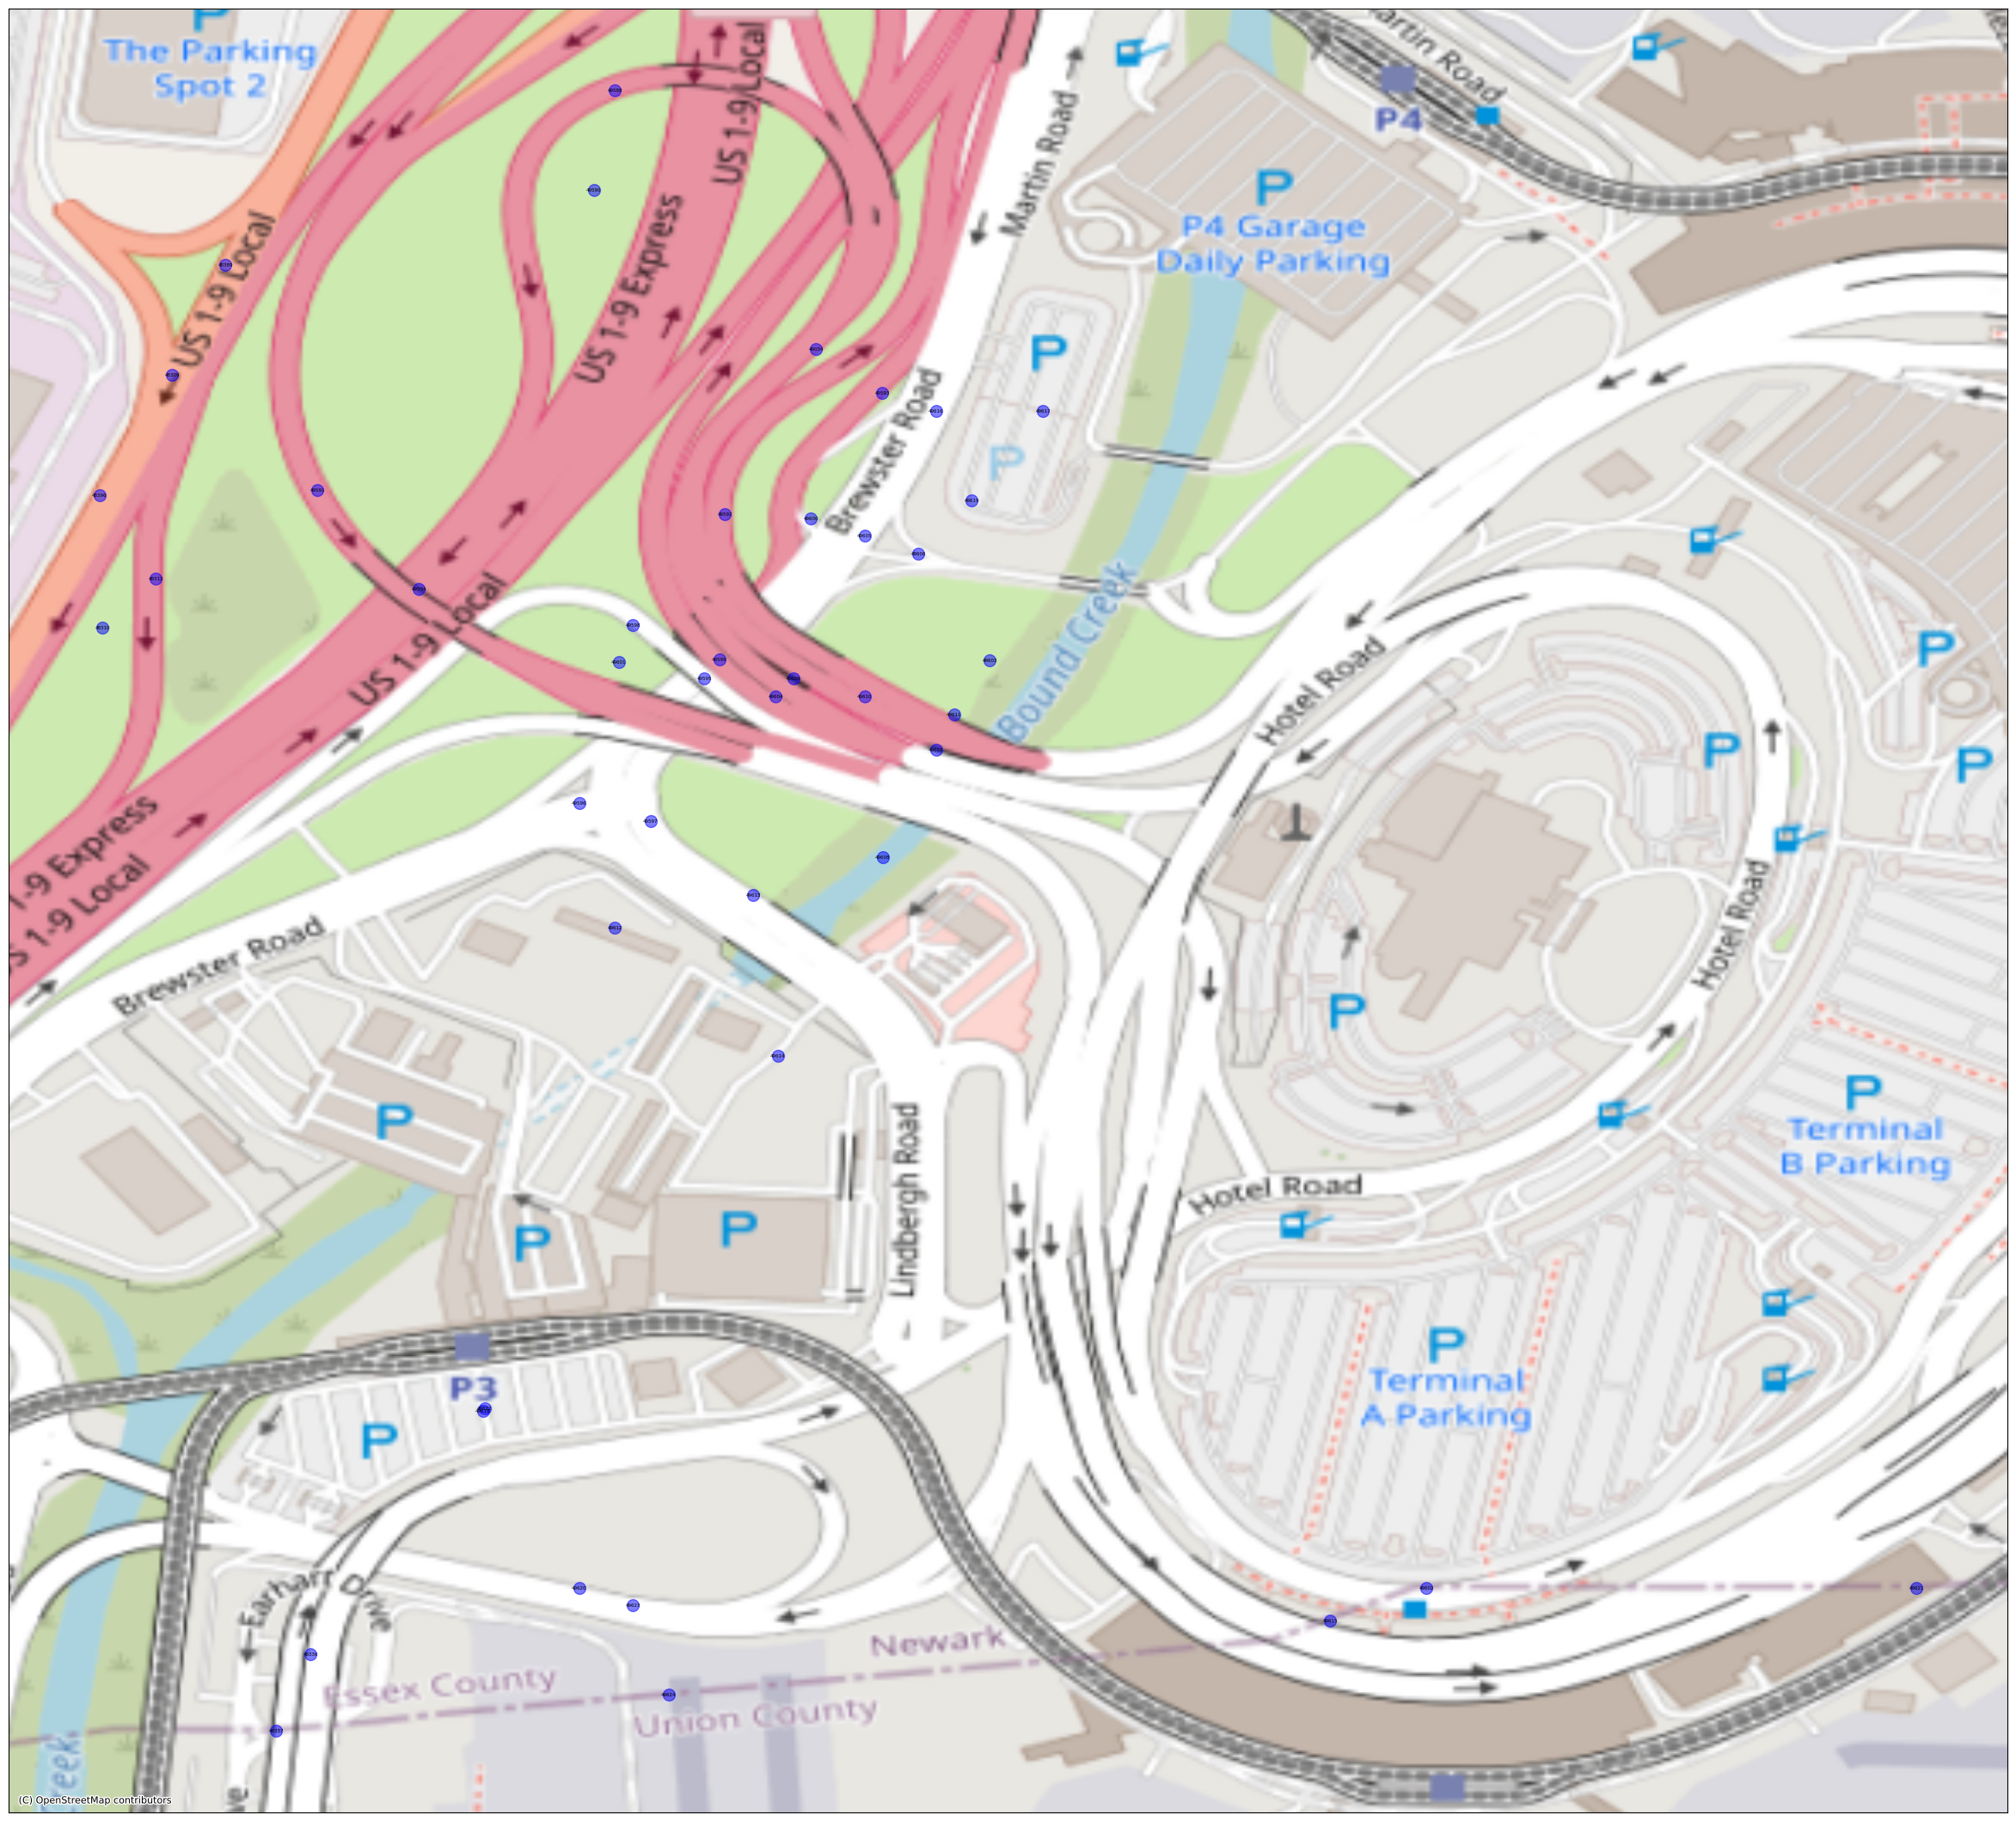
\includegraphics[width=3cm]{newark}
    \caption{NewArk}
    \label{fig:newark}
\end{figure}

\begin{figure}[htbp]
    \centering
    \includegraphics[width=3cm]{jfk-laguardia}
    \caption{JFK - LaGuardia}
    \label{fig:jfk-laguardia}
\end{figure}

\begin{figure}[htbp]
    \centering
    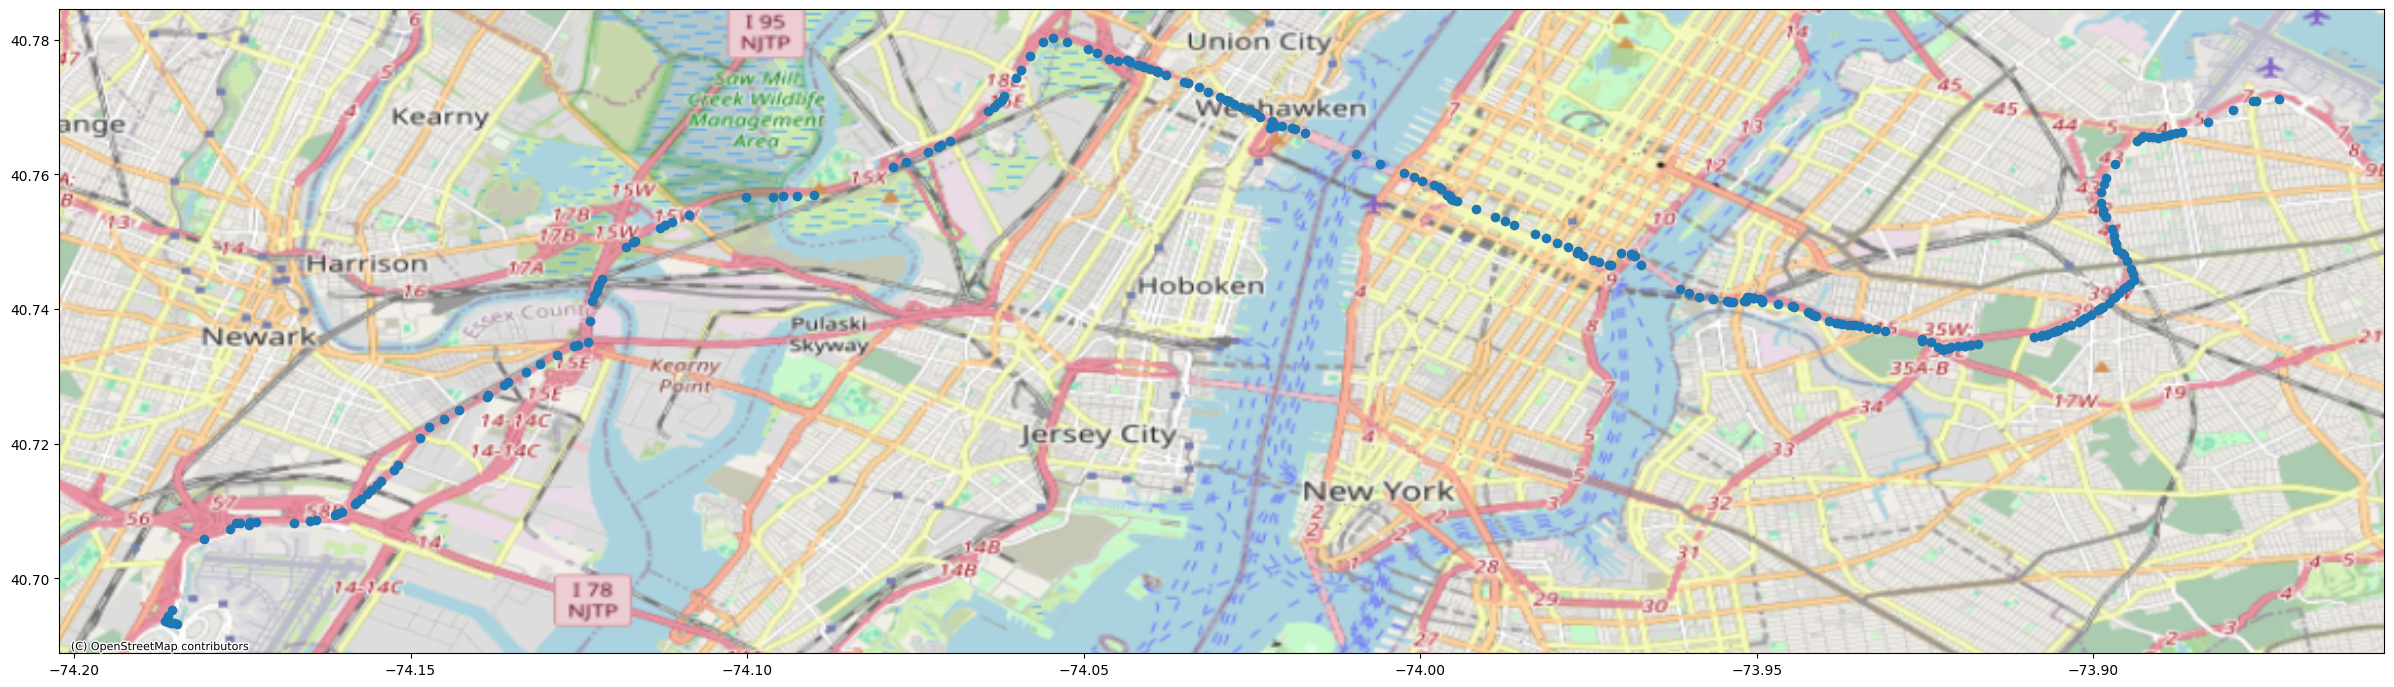
\includegraphics[width=3cm]{laguardia-newark}
    \caption{LaGuardia - NewArk}
    \label{fig:laguardia-newark}
\end{figure}

\begin{figure}[htbp]
    \centering
    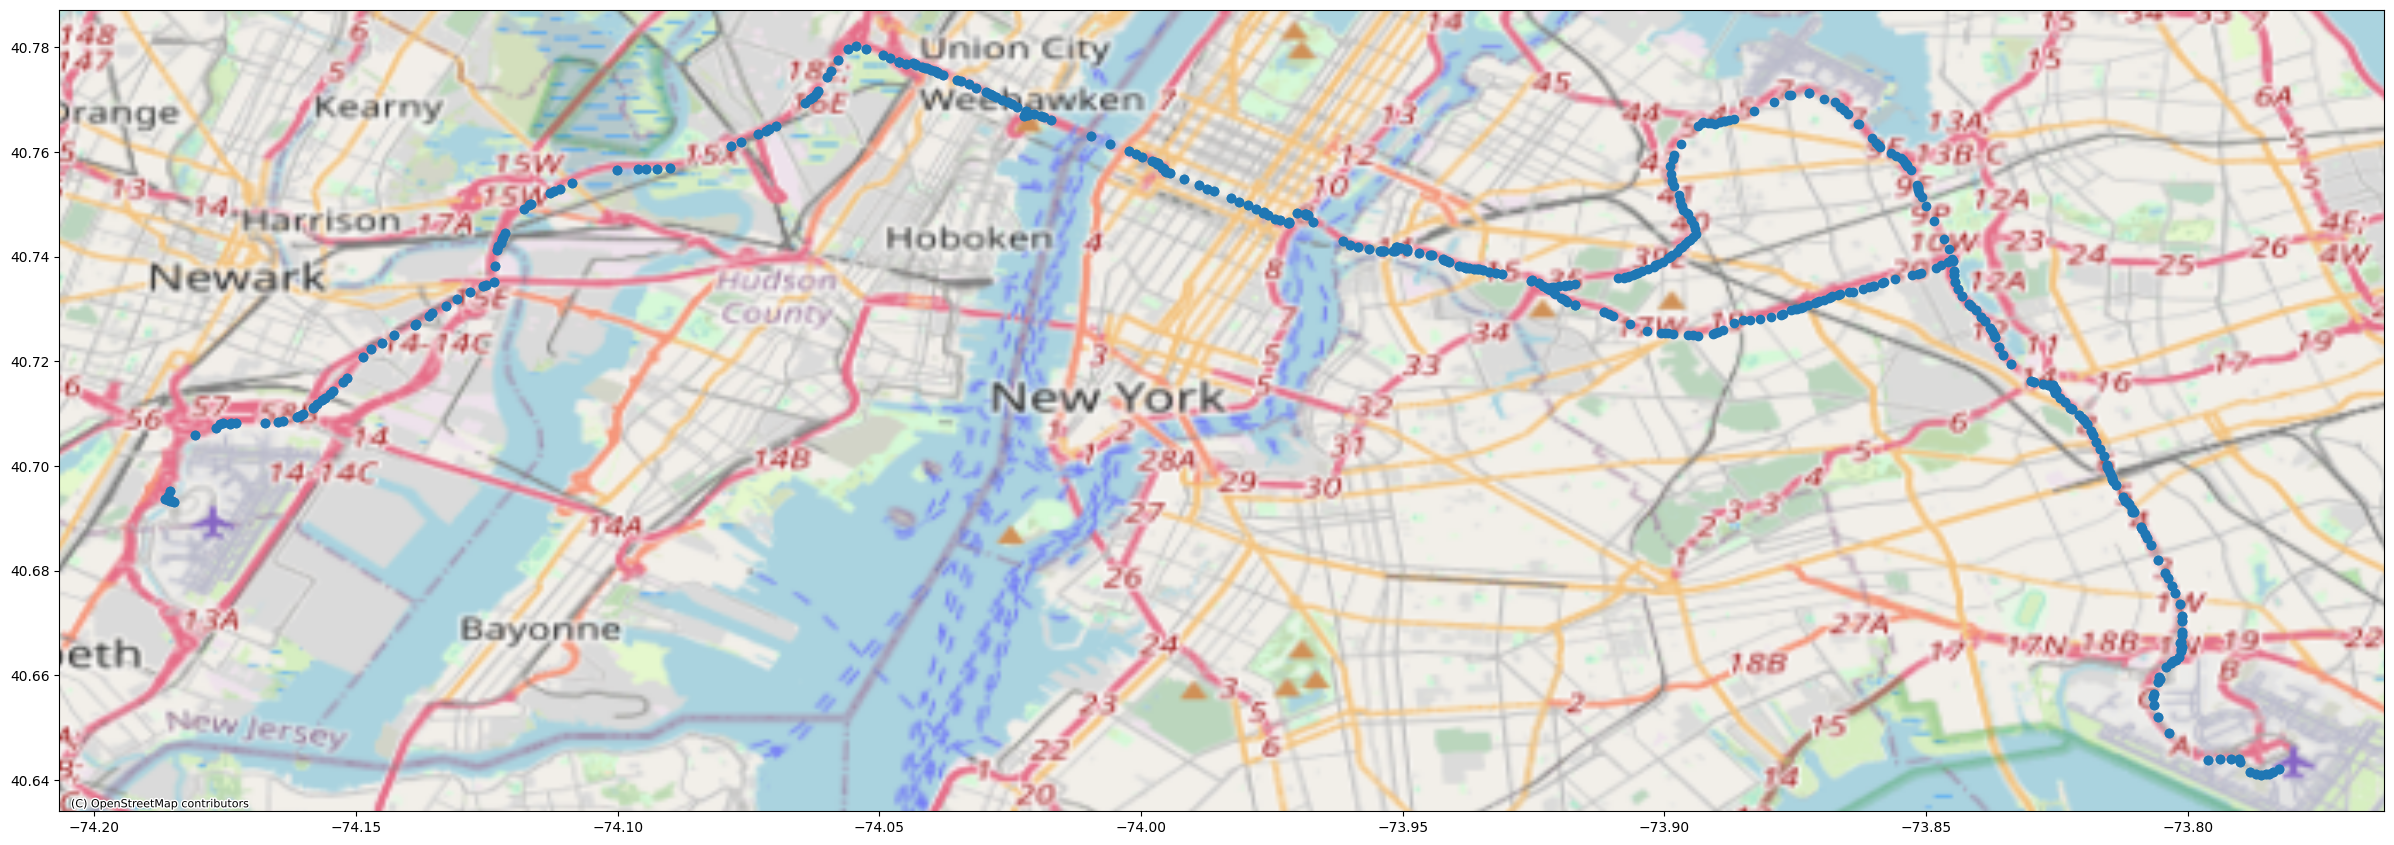
\includegraphics[width=3cm]{roundtrip}
    \caption{Roundtrip}
    \label{fig:roundtrip}
\end{figure}
\newpage

\chapter{Legal}
Die Ausarbeitung der Aufgabe wurde durch \texttt{OpenAI - GPT-4.5 Turbo}, \texttt{OpenAI - GPT-4.5 Vision}, \texttt{OpenAI - GPT-4o}, \texttt{Anthropic -- Claude 3 Opus},  \texttt{Kagi - FastGPT} mit mehreren unterschiedlichen Prompts und Custom Instructions unterstützt.

\end{document}